\documentclass[11pt]{article}
\usepackage[margin=2.5cm]{geometry}
\usepackage{pgfplots}\pgfplotsset{compat=1.17}
\begin{document}
\begin{center}{\Large\bfseries Image Classification: A Complete Lab Report}\\[4pt]Sample Student\end{center}
\section{Introduction}
Convolutional networks and vision transformers are the two families most often compared in
introductory deep learning courses. This report follows the official lab handout and compares one
model of each family on two datasets.
\section{Setup}
All models were trained for 20 epochs on 4 GPUs with a batch size of 256. The learning rate was reduced by 10\% every 5 epochs. Images were normalised with the usual channel statistics.
\section{Results}
Figs.~\ref{fig:acc} and~\ref{fig:loss} summarise training.
\begin{figure}[h]\centering
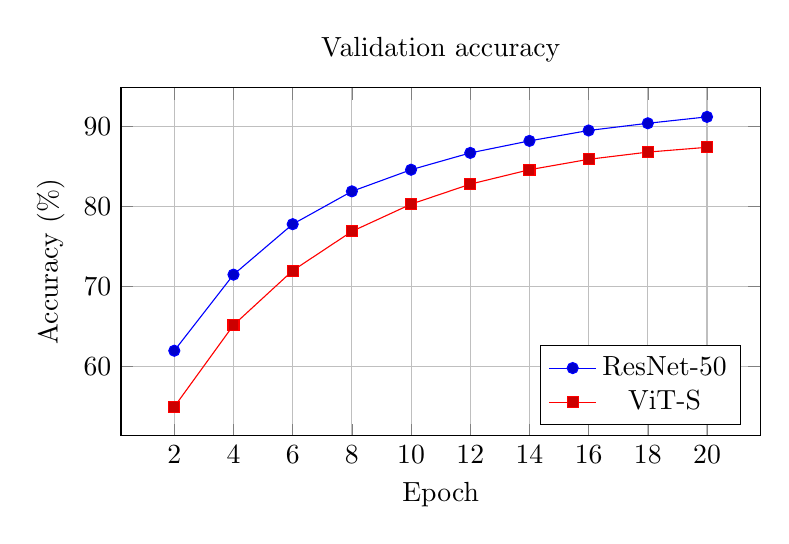
\begin{tikzpicture}\begin{axis}[width=0.8\textwidth,height=6cm,xlabel={Epoch},ylabel={Accuracy (\%)},title={Validation accuracy},xtick={2,4,6,8,10,12,14,16,18,20},legend pos=south east,grid=major]
\addplot+[mark=*] coordinates {(2,62.0) (4,71.5) (6,77.8) (8,81.9) (10,84.6) (12,86.7) (14,88.2) (16,89.5) (18,90.4) (20,91.2)}; \addlegendentry{ResNet-50}
\addplot+[mark=square*] coordinates {(2,55.0) (4,65.2) (6,72.0) (8,76.9) (10,80.3) (12,82.8) (14,84.6) (16,85.9) (18,86.8) (20,87.4)}; \addlegendentry{ViT-S}\end{axis}\end{tikzpicture}
\caption{Validation accuracy. ResNet-50 reaches 91.2\% at epoch 20.}\label{fig:acc}\end{figure}
ResNet-50 achieved 91.2\% validation accuracy at epoch 20. ViT-S reached 90.0\% validation accuracy at epoch 20. At epoch 10, ViT-S is 4.3 points lower than ResNet-50.
\begin{figure}[h]\centering
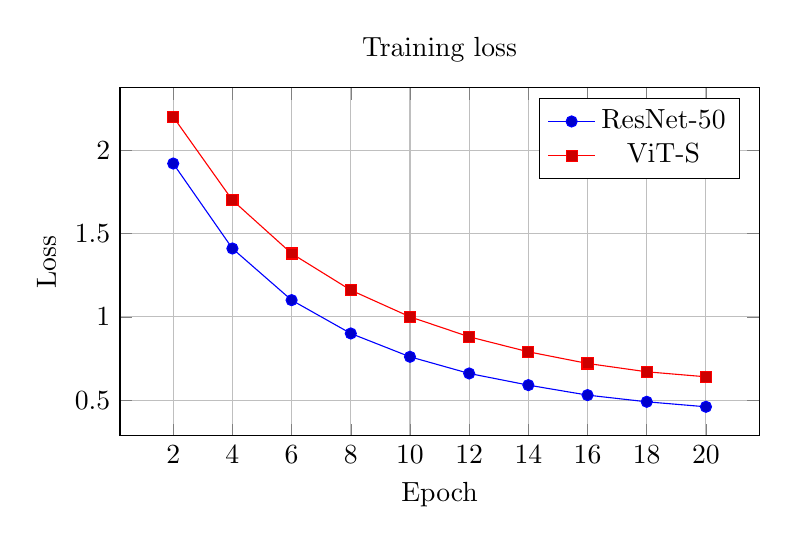
\begin{tikzpicture}\begin{axis}[width=0.8\textwidth,height=6cm,xlabel={Epoch},ylabel={Loss},title={Training loss},xtick={2,4,6,8,10,12,14,16,18,20},legend pos=north east,grid=major]
\addplot+[mark=*] coordinates {(2,1.92) (4,1.41) (6,1.1) (8,0.9) (10,0.76) (12,0.66) (14,0.59) (16,0.53) (18,0.49) (20,0.46)}; \addlegendentry{ResNet-50}
\addplot+[mark=square*] coordinates {(2,2.2) (4,1.7) (6,1.38) (8,1.16) (10,1.0) (12,0.88) (14,0.79) (16,0.72) (18,0.67) (20,0.64)}; \addlegendentry{ViT-S}\end{axis}\end{tikzpicture}
\caption{Training loss.}\label{fig:loss}\end{figure}
From epoch 2 to epoch 20, the training loss of ViT-S fell by 71\%. The training loss of ResNet-50 is 0.46 at epoch 20.
\begin{figure}[h]\centering
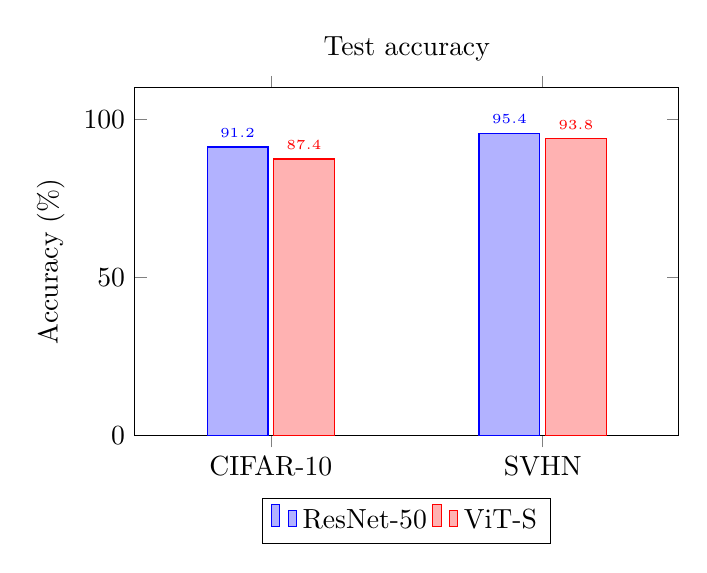
\begin{tikzpicture}\begin{axis}[ybar,width=0.7\textwidth,height=6cm,ymin=0,ymax=110,bar width=22pt,enlarge x limits=0.5,symbolic x coords={CIFAR-10,SVHN},xtick=data,ylabel={Accuracy (\%)},title={Test accuracy},legend style={at={(0.5,-0.18)},anchor=north,legend columns=-1},nodes near coords,every node near coord/.append style={font=\tiny}]
\addplot coordinates {(CIFAR-10,91.2) (SVHN,95.4)}; \addlegendentry{ResNet-50}
\addplot coordinates {(CIFAR-10,87.4) (SVHN,93.8)}; \addlegendentry{ViT-S}\end{axis}\end{tikzpicture}
\caption{Test accuracy on CIFAR-10 and SVHN.}\label{fig:bar}\end{figure}
On SVHN, ViT-S achieves 93.8\% test accuracy. On CIFAR-10, ResNet-50 is 6.0 points better than ViT-S.
\section{Discussion}
ViT-S does not reach the accuracy of ResNet-50 at any epoch, staying below 88\%. ResNet-50 achieved 91.2\% validation accuracy at epoch 20. Overall the convolutional network remains the stronger choice
for small datasets, in line with the literature.
\end{document}
